\documentclass[11pt,a4paper]{article}

\usepackage[margin=2.5cm]{geometry}
\usepackage[T1]{fontenc}
\usepackage[utf8]{inputenc}
\usepackage{lmodern}
\usepackage{microtype}
\usepackage{graphicx}
\usepackage{booktabs}
\usepackage{xcolor}
\usepackage[hidelinks]{hyperref}
\usepackage{xurl}
\usepackage[nameinlink]{cleveref}

\graphicspath{{figures/}}

\title{Fashion Search Engine\\[0.3em]\large Part 1: Text Processing and Exploratory Data Analysis}
\author{Marc Mallol\and Èric Dürr\and Oriol Pont}
\date{Information Retrieval and Web Analytics, 2026}

\begin{document}
\maketitle

\section{Introduction}

This report covers Part 1 of our fashion search engine: text processing and
exploratory data analysis of a catalogue of 28{,}080 products from Flipkart, an
Indian e-commerce site. Each product has a title, an optional description, a
brand, a category and sub-category, a list of product details (fabric, sleeve,
colour, \ldots), a seller, prices, a discount, an average rating, a stock flag
and a URL. The goal of this part is to turn the raw catalogue into clean records
that the later parts index (Part~2), rank (Part~3) and serve through a RAG web
application (Part~4).

Section~2 describes the data preparation: the text pre-processing pipeline, the
fields kept for each result, and how categorical and numerical fields are
handled. We check each decision against the two validation queries in
\path{validation_labels.csv}, \emph{women full sleeve sweatshirt cotton} and
\emph{men slim jeans blue}. Section~3 explores the text and the products of the
catalogue, and Section~4 summarises what this means for the search engine.

The code is at \url{https://github.com/uripont/fashion-search-engine}, tag
\texttt{IRWA-2026-part-1}. The \path{fashion_search} package holds the reusable
code, and \path{notebooks/part_1.ipynb} runs it and produces every number and
figure in this report. The README explains how to reproduce them.

\section{Data preparation}

The code is in the \path{fashion_search} package: \path{text.py} turns text into
search terms and \path{corpus.py} builds the product records. Section~2 of
\path{notebooks/part_1.ipynb} runs them and holds the evidence for each decision.
Together they turn each of the 28{,}080 products into one record that keeps every
field a result must show, with numbers parsed, plus one list of terms per searchable
field. The records are saved to \path{data/processed/products.parquet}, which the
next parts of the project read.

\subsection{Text pre-processing}

The same function, \texttt{build\_terms}, processes every text field and every
query, so query terms and document terms always match. It applies, in order:

\begin{enumerate}
  \item \textbf{Repair and normalize.} 91 descriptions contain UTF-8 text that was
    decoded as Latin-1 (\texttt{â\textbackslash x80\textbackslash x99} instead of an
    apostrophe), and 6{,}817 titles contain non-breaking spaces. We undo the former,
    fold accents and special spaces to plain ASCII and lowercase everything.
  \item \textbf{Unify spelling variants.} The catalogue writes the same garment as
    \emph{t-shirt}, \emph{t shirt}, \emph{tshirt} and \emph{tee}; all become
    \emph{tshirt}. \emph{v-neck} and \emph{v neck} become \emph{vneck}, and glued
    words such as \emph{slimfit} are split (\emph{slim fit}).
  \item \textbf{Possessives and hyphens.} \emph{women's} becomes \emph{women}, so it
    matches the query word; hyphenated words are joined (\emph{round-neck} becomes
    \emph{roundneck}).
  \item \textbf{Remove punctuation.} Every other symbol becomes a space. Removing it
    instead would glue words that the source writes without a space after a full
    stop (\emph{cotton.Designed}).
  \item \textbf{Tokenize} with NLTK's \texttt{word\_tokenize}~\cite{bird2009nltk}.
  \item \textbf{Remove stop words, numbers and single letters,} using NLTK's English
    stop word list. Gender words (\emph{men}, \emph{women}) are not in it and are kept,
    since both validation queries depend on them.
  \item \textbf{Stem} with the Porter stemmer (\emph{sleeves} and \emph{sleeve} become
    \emph{sleev}). Lemmatization would give readable terms, but it needs
    part-of-speech tags to be accurate and merges fewer variants.
\end{enumerate}

\subsection{Fields returned for each result}

All fourteen fields a result must show are kept in their original form: \texttt{pid}
(the key used for evaluation), \texttt{title}, \texttt{description}, \texttt{brand},
\texttt{category}, \texttt{sub\_category}, \texttt{product\_details}, \texttt{seller},
\texttt{out\_of\_stock}, \texttt{selling\_price}, \texttt{discount},
\texttt{actual\_price}, \texttt{average\_rating} and \texttt{url}. The term lists are
added next to them, never in their place, so a result page can show the original
text. Empty strings are stored as missing values, so a result can leave out what a
product does not have. Many fields are often missing
(\cref{tab:presence}); most importantly, 40\% of products have no description.

\begin{table}[htbp]
  \centering
  \begin{tabular}{lr@{\hskip 2em}lr}
    \toprule
    Field & Present & Field & Present \\
    \midrule
    description & 60.3\% & average\_rating & 91.9\% \\
    brand & 92.8\% & discount & 97.0\% \\
    seller & 94.1\% & actual\_price & 97.2\% \\
    \bottomrule
  \end{tabular}
  \caption{Fields that are often missing. \texttt{selling\_price} is missing in only
    2 products; the other seven fields are present in every product.}
  \label{tab:presence}
\end{table}

\subsection{Categorical fields}

There are three ways to handle \texttt{category}, \texttt{sub\_category},
\texttt{brand}, \texttt{product\_details} and \texttt{seller}:

\begin{itemize}
  \item \textbf{Merge them into one text field.} It is simple, and a query matches
    whatever field a word is in. But a match in a generic field counts as much as a
    match in the title, and the field's statistics are mixed together. For example,
    \emph{clothing} would appear in 97\% of products and say nothing.
  \item \textbf{Index them as separate fields.} The ranking can weight each field
    differently (a title match is stronger evidence than a description match) and
    each keeps its own term statistics. It costs one index per field and more
    complex queries.
  \item \textbf{Use them as filters.} Exact values, chosen by the user or detected in
    the query, restrict the results without affecting the text score. This only works
    for fields with few, well-defined values.
\end{itemize}

We chose by looking at where the words of the two validation queries appear in the
products judged relevant (\cref{fig:query-terms}). \emph{Cotton} never appears in a
title: it is only in the description or in the Fabric detail. \emph{Full} and
\emph{sleeve} are in the Sleeve detail of every relevant product. \emph{Blue} and
\emph{men} are in Color and Ideal For. No query word ever appears in brand,
category or sub-category. Because queries are conjunctive, a product is found only if
\emph{every} query word is indexed: with titles and descriptions alone, 11 of the
13 relevant products for query~1 are found, and adding the product details finds all
13.

\begin{figure}[htbp]
  \centering
  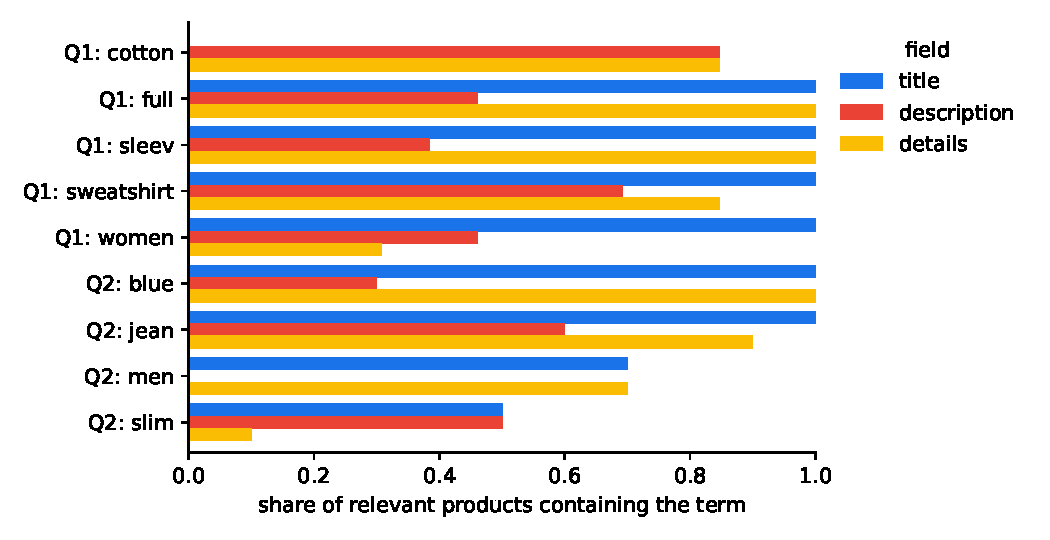
\includegraphics[width=0.9\linewidth]{query_terms_by_field.pdf}
  \caption{Share of relevant products for each validation query that contain each
    (stemmed) query term, by field. Brand and category contain none of them.}
  \label{fig:query-terms}
\end{figure}

Our decision, field by field:

\begin{itemize}
  \item \textbf{Title, description, product details and brand are indexed as separate
    text fields.} A plain inverted index can still use all of them together (a
    document's terms are the union of the four), while later ranking can weight them
    separately. From \texttt{product\_details} we index the \emph{values} (\emph{Cotton
    Blend}, \emph{Full Sleeve}, \emph{Slim}) but not the keys, which repeat in almost
    every product. We drop \emph{Style Code}, an internal product code. Brand is
    distinctive (324 brands; the most common has only 3.6\% of products), so a query
    naming a brand should find it, although many brand names are truncated in the
    source data (\cref{sec:catalogue}).
  \item \textbf{Category and sub-category are filters.} There are only 4 categories,
    and 96.6\% of products are \emph{Clothing and Accessories}; there are 24
    sub-categories, and \emph{Topwear} alone has 54.5\%. As text they would add an
    almost constant word to every product; as filters (\emph{Footwear} only) they are
    precise.
  \item \textbf{Seller is a filter and is displayed, not searched.} Its 534 values are
    company names that do not describe the product, so they would match unrelated
    queries.
\end{itemize}

The second validation query shows the limits of conjunctive queries: whatever fields
are indexed, only 6 of its 10 relevant products contain \emph{slim}, since the
others are \emph{tapered} or \emph{super skinny} jeans that the judges still found
relevant. Some identical products are also judged differently, so the labels contain
some noise. We return to this in Part 2.

\subsection{Numerical fields}

\texttt{selling\_price}, \texttt{actual\_price}, \texttt{discount} and
\texttt{average\_rating} arrive as text (\texttt{"2,999"}, \texttt{"69\% off"},
\texttt{"3.9"}). We parse them into numbers and keep missing values as missing, not
as zero, which would make a product look free or badly rated
(\cref{tab:numeric}). \texttt{out\_of\_stock} is already a boolean. Two checks confirm the parsing: no selling price is above its actual
price, and every parsed discount is within one percentage point of the one implied by
the two prices.

\begin{table}[htbp]
  \centering
  \begin{tabular}{lrrrr}
    \toprule
    Field & Min & Median & Max & Missing \\
    \midrule
    selling\_price (INR) & 99 & 545 & 7{,}999 & 2 \\
    actual\_price (INR) & 150 & 1{,}199 & 12{,}999 & 777 \\
    discount (\%) & 1 & 53 & 87 & 855 \\
    average\_rating & 1.0 & 3.8 & 5.0 & 2{,}261 \\
    \bottomrule
  \end{tabular}
  \caption{Numerical fields after parsing.}
  \label{tab:numeric}
\end{table}

These fields are \textbf{not indexed as text terms}. A term only helps if users type
it, and nobody searches for \emph{921}. Each price would also become its own rare
term, so TF-IDF would give it a high weight, and as text it could not express
\emph{under 1{,}000}. Kept as numbers, they serve three purposes: filters (price range,
minimum rating, in stock only), signals for our own ranking score in Part 3 (a
well-rated, discounted, available product is a better result), and information on the
results page.

\section{Exploratory data analysis}

Section~3 of the notebook produces every figure below.

\subsection{Text}

\paragraph{Length.} Titles are short and uniform: 6.5 words on average (median 6,
maximum 38). Descriptions are longer and far more variable: 29.8 words on
average, but 40\% of products have none, so the median is only 10, and the
longest has 623 words (\cref{fig:wordcount}). Titles are noun phrases, not
sentences. Splitting descriptions into sentences with NLTK gives 3.1 sentences of
15.7 words on average (medians 2 and 14): short marketing blurbs rather than long
text. This is approximate, because some descriptions omit the space after a full
stop, and those sentence pairs count as one. Since every product has a title and only 60\% have a
description, the title is the one field we can rely on for every product.

\begin{figure}[htbp]
  \centering
  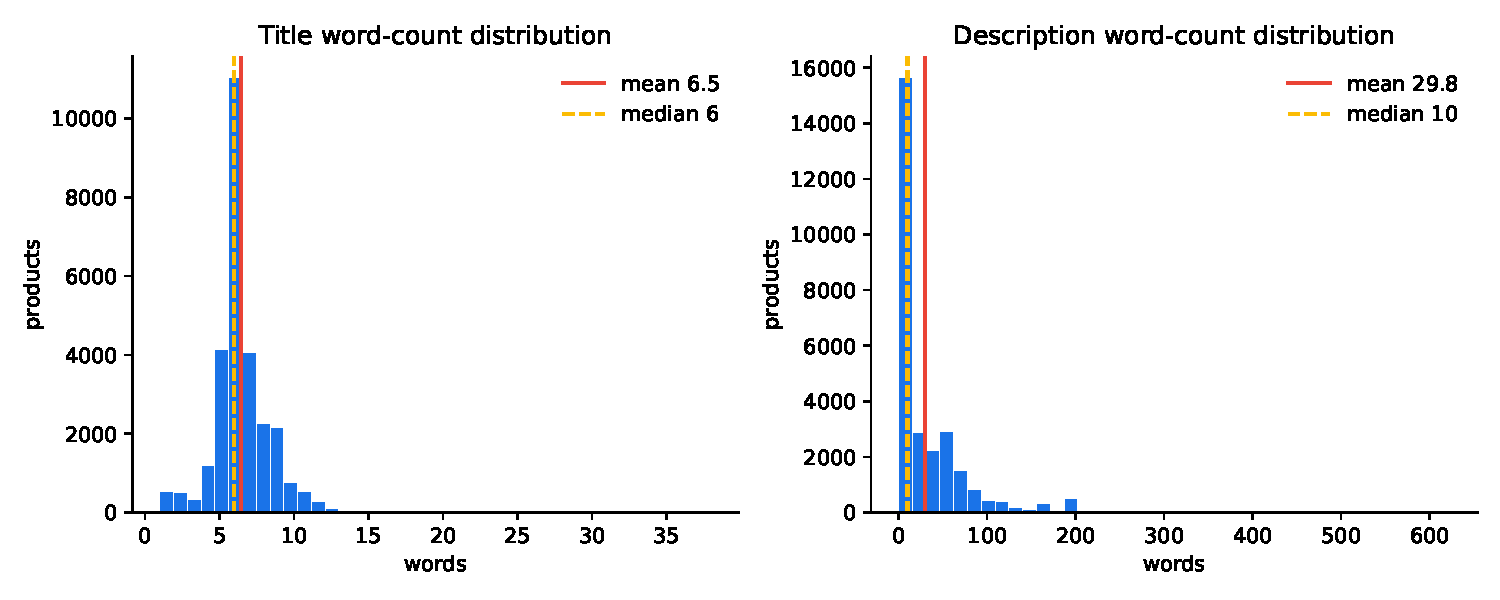
\includegraphics[width=\linewidth]{word_count_distribution.pdf}
  \caption{Words per title and per description (raw text).}
  \label{fig:wordcount}
\end{figure}

\paragraph{Vocabulary.} Counting lowercase whitespace-separated words, titles use
953 distinct words and descriptions 10{,}250. Pre-processing reduces them to 652
(\(-32\%\)) and 4{,}933 (\(-52\%\)) terms (\cref{fig:vocab}); product details add
3{,}604 terms and brands 388. Titles share a tiny vocabulary because they follow a
template (pattern, gender, neck, colour, garment, as in \emph{Printed Women Round
Neck Black T-Shirt}), so many products have nearly identical titles.

\begin{figure}[htbp]
  \centering
  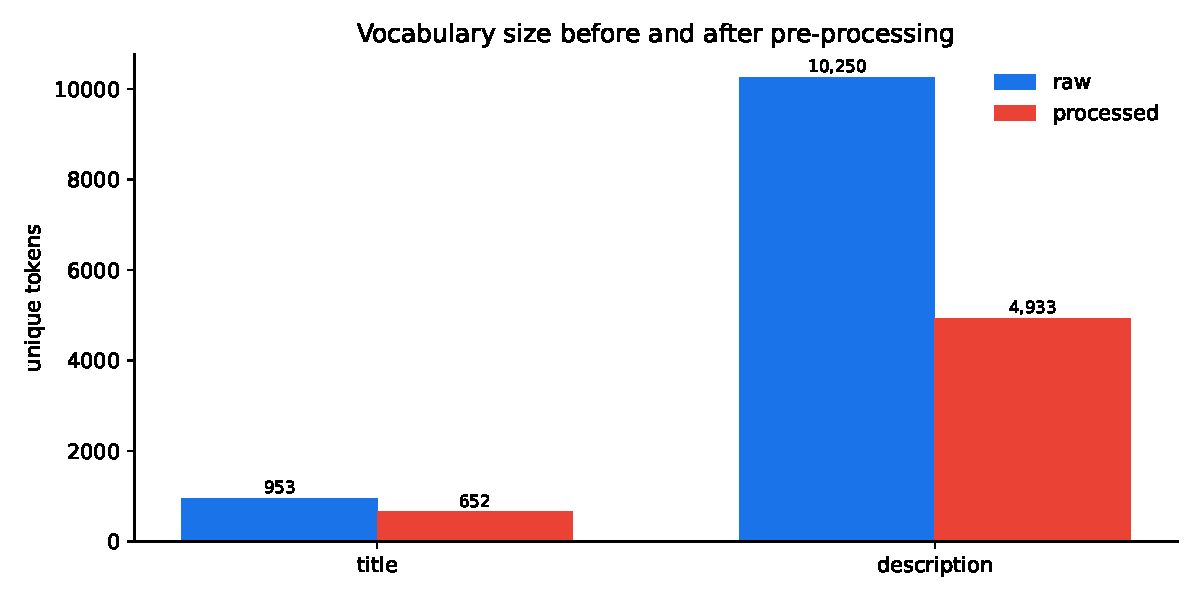
\includegraphics[width=0.65\linewidth]{vocabulary_size.pdf}
  \caption{Vocabulary size per field, before and after pre-processing.}
  \label{fig:vocab}
\end{figure}

\paragraph{Frequent terms.} The catalogue is dominated by t-shirts:
\emph{tshirt} is the most frequent term in titles and descriptions (28{,}256
occurrences), followed by \emph{women} (17{,}569), \emph{men} (16{,}831),
\emph{neck}, \emph{print} and \emph{cotton} (\cref{fig:top50,fig:clouds}). Several
words of the validation queries (\emph{women}, \emph{men}, \emph{cotton},
\emph{sleev}, \emph{blue}) are among the most frequent terms. They appear in so
many products that they barely tell them apart, so TF-IDF will give them low
weight and the rarer garment words (\emph{sweatshirt}, \emph{jean}) will drive
the ranking.

\begin{figure}[htbp]
  \centering
  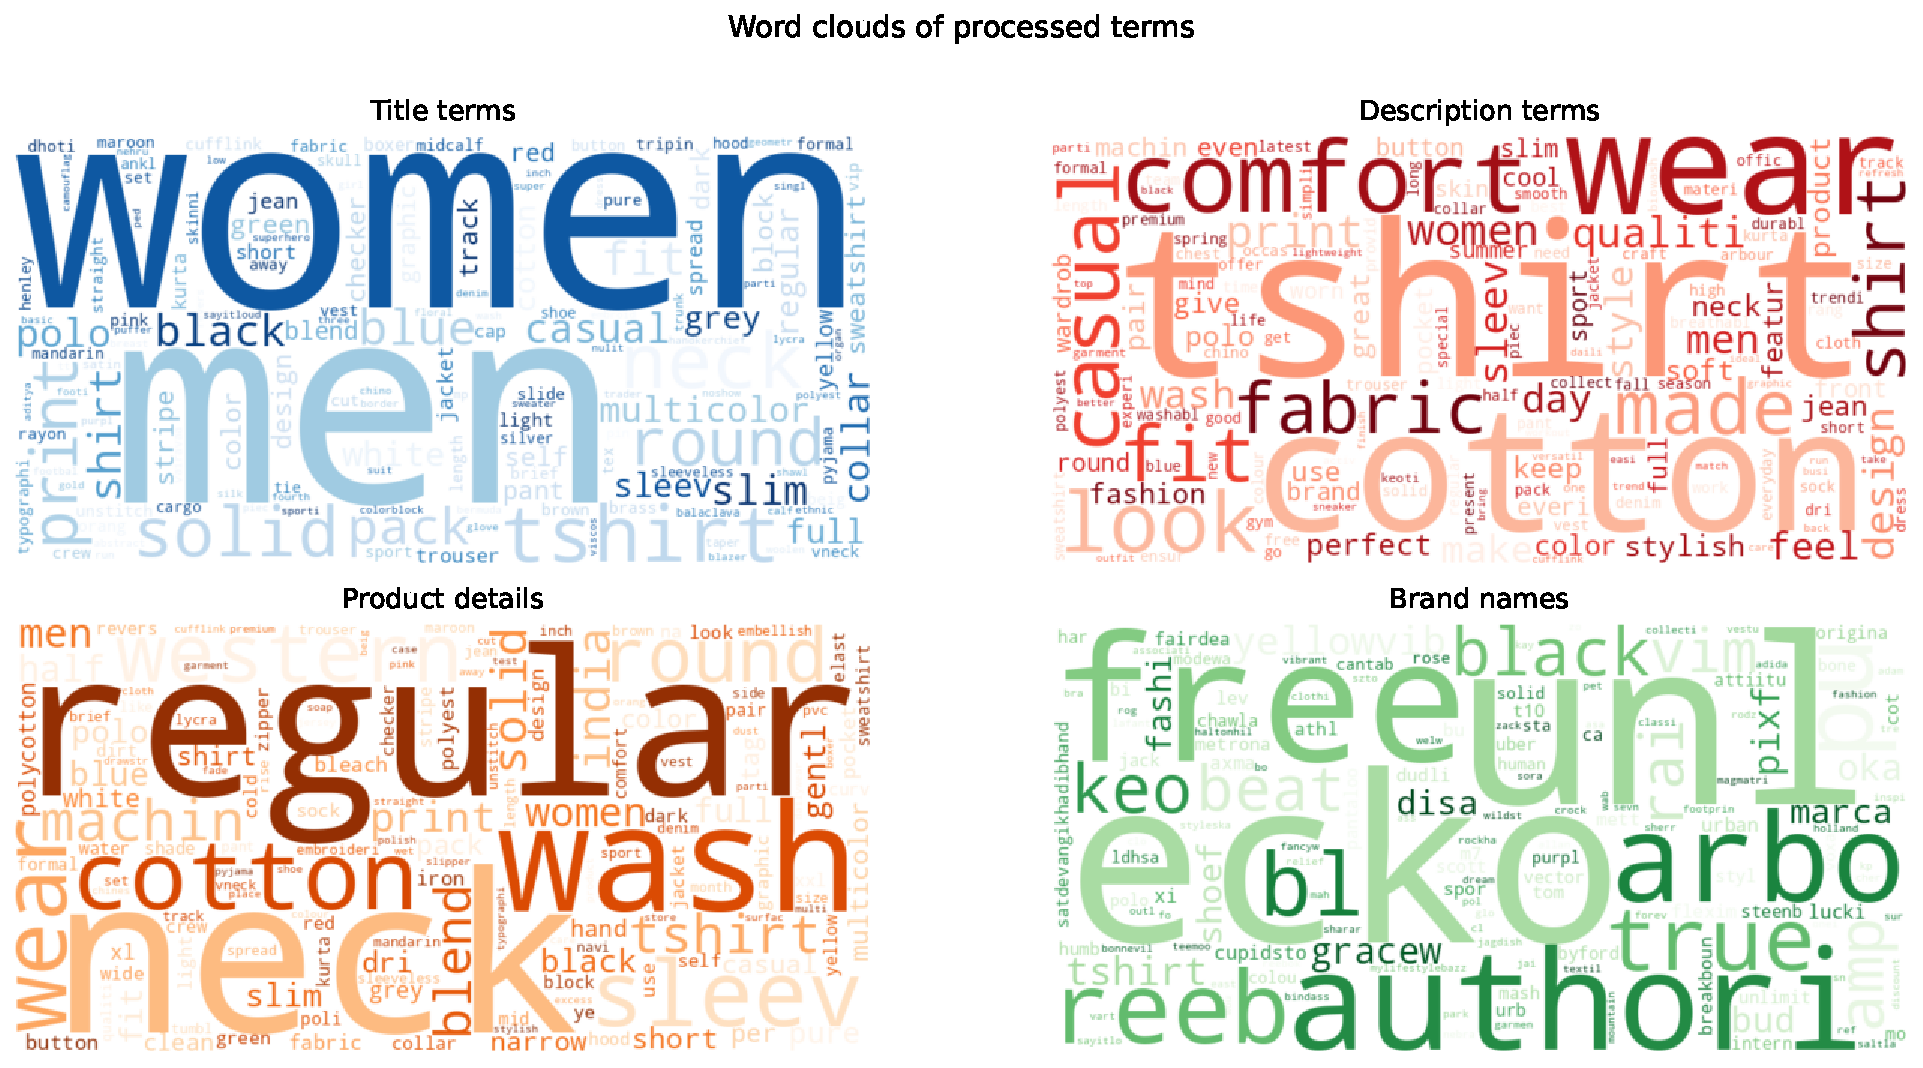
\includegraphics[width=\linewidth]{word_clouds.pdf}
  \caption{Most frequent terms per field, after pre-processing.}
  \label{fig:clouds}
\end{figure}

\begin{figure}[htbp]
  \centering
  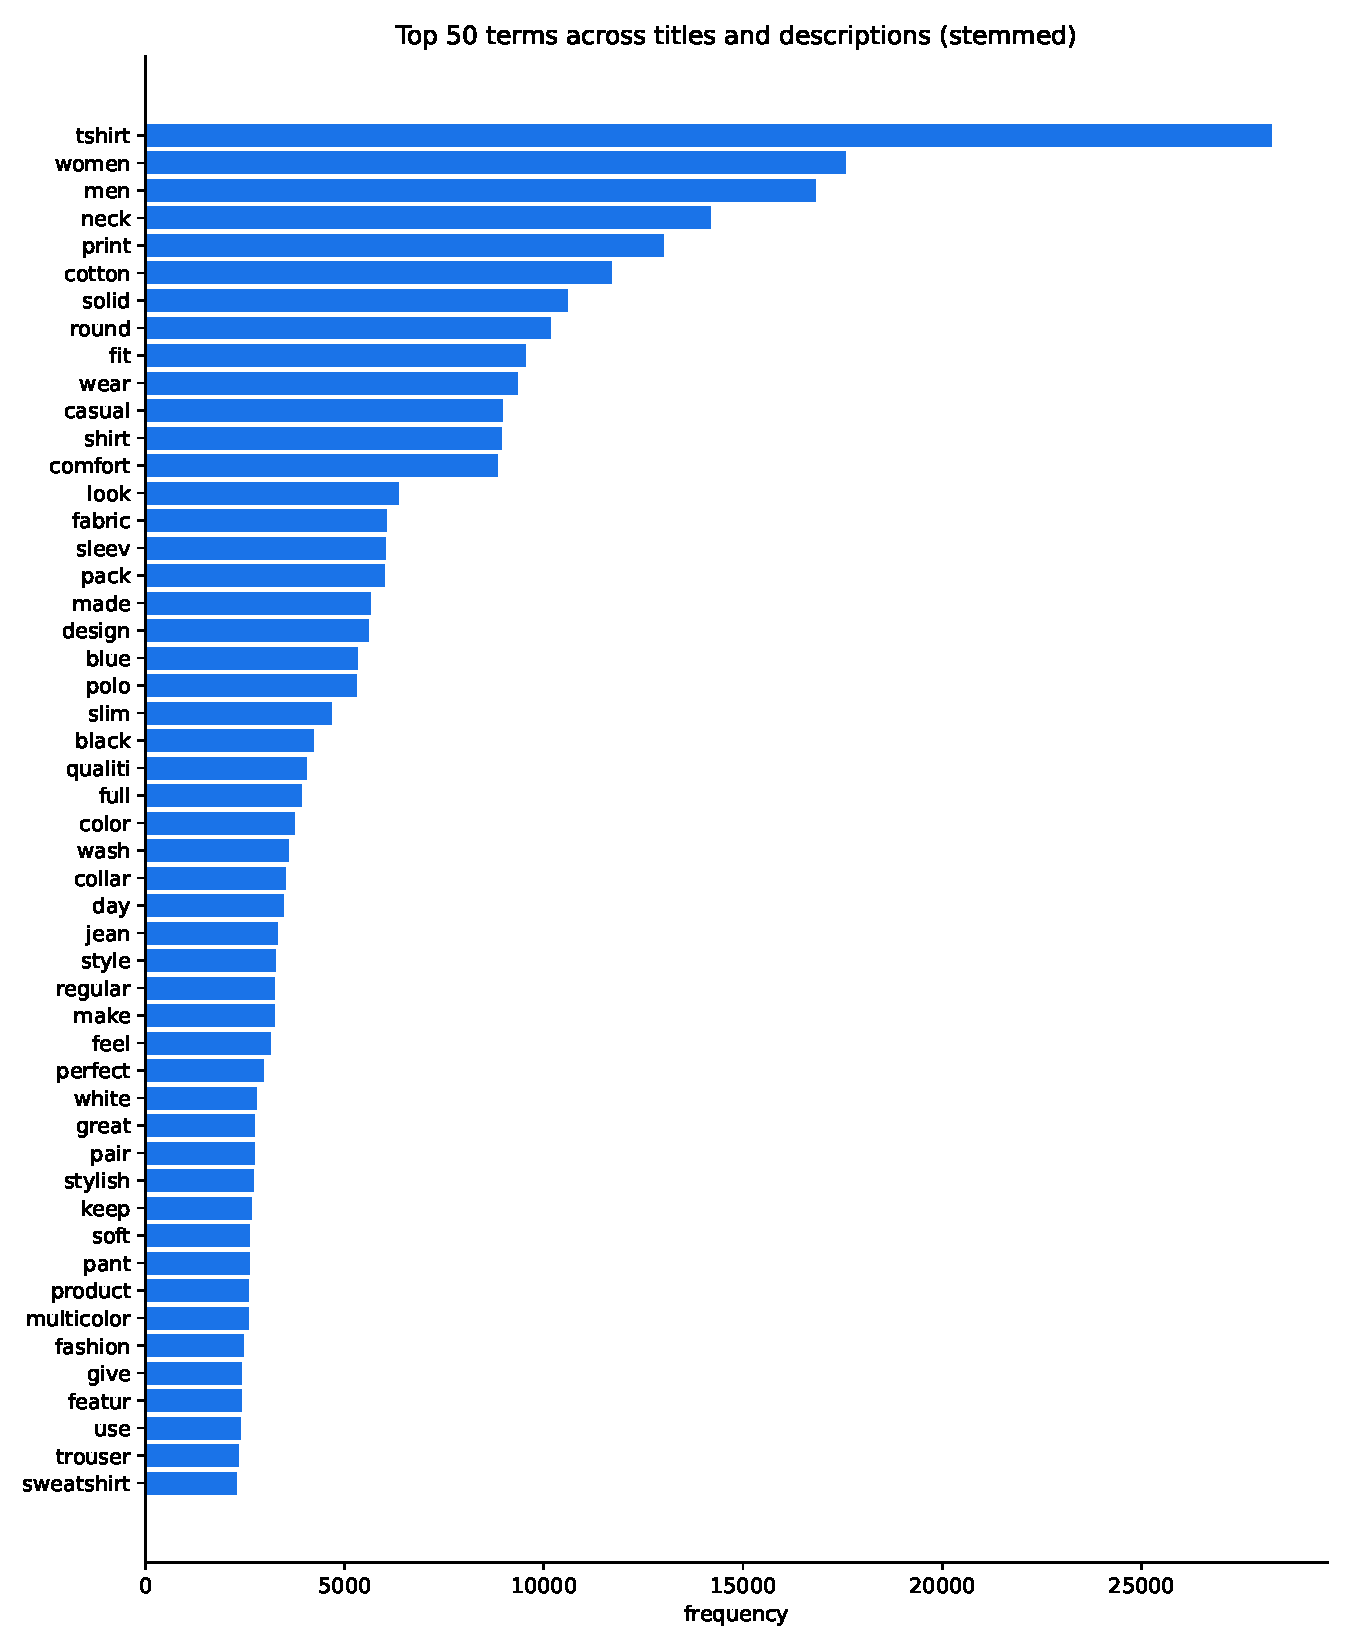
\includegraphics[width=0.55\linewidth]{top50_terms.pdf}
  \caption{The 50 most frequent terms in titles and descriptions (stemmed).}
  \label{fig:top50}
\end{figure}

\paragraph{Named entities.} We ran spaCy's \texttt{en\_core\_web\_sm}
model~\cite{honnibal2020spacy} on a random sample of 2{,}000 titles. It finds an
entity in 1{,}402 of them, 1{,}772 in total (ORG 930, PERSON 421, CARDINAL 378),
but nearly all are wrong
(\cref{fig:ner}): \emph{Solid Women} is tagged as a person, whole titles such as
\emph{Printed Women Round Neck Black T-Shirt} as organisations, \emph{Kurta} as a
place, and the CARDINAL entities are pack sizes. The model, trained on news text,
reads capitalised product titles as names. The real entities, brands, already
have their own field, so we do not use entity recognition for indexing.

\begin{figure}[htbp]
  \centering
  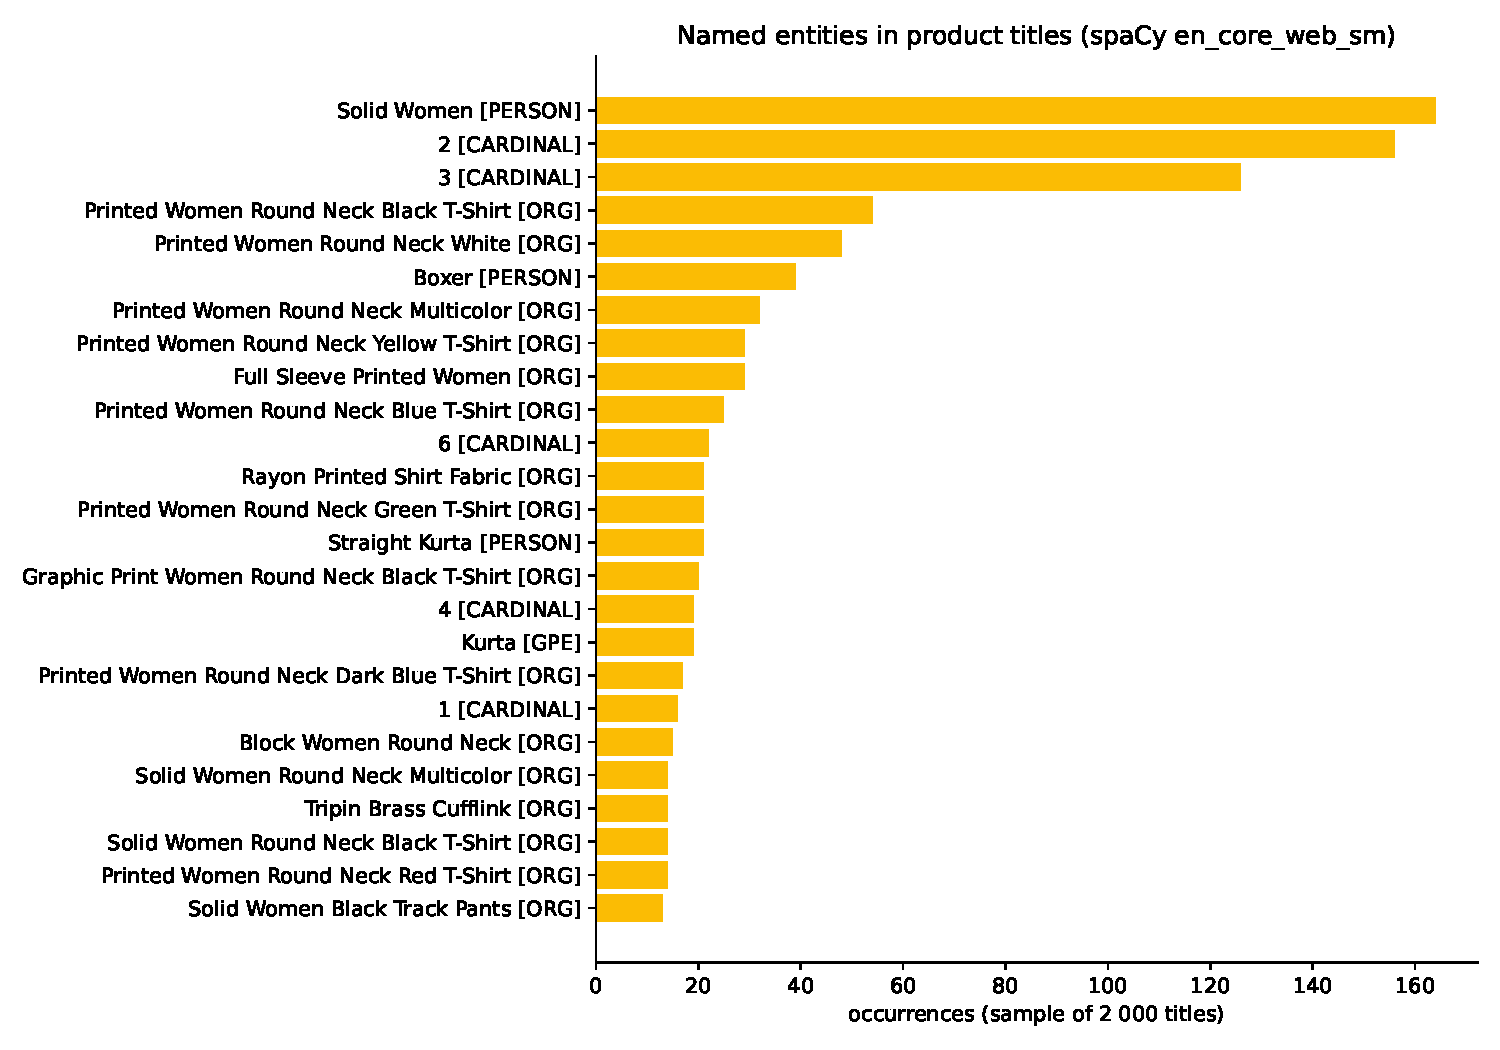
\includegraphics[width=0.8\linewidth]{named_entities.pdf}
  \caption{The 25 most frequent named entities in a sample of 2{,}000 titles.}
  \label{fig:ner}
\end{figure}

\subsection{Catalogue}
\label{sec:catalogue}

\paragraph{Categories.} 96.6\% of products are \emph{Clothing and Accessories};
the rest are mostly \emph{Footwear}, with only a handful of \emph{Bags, Wallets
\& Belts} and \emph{Toys} (\cref{fig:categories}). \emph{Topwear} alone holds
54.5\% of products, followed by \emph{Bottomwear} and \emph{Winter Wear}. Some
sub-category values are noisy, with a brand glued to a category name
(\emph{Uber Urban Clothing and Accessories}) or the same value in two spellings
(\emph{SUNSHOPPING} and \emph{Sunshopping Bags, Wallets \& Belts}); they are rare,
but a category filter has to account for them.

\begin{figure}[htbp]
  \centering
  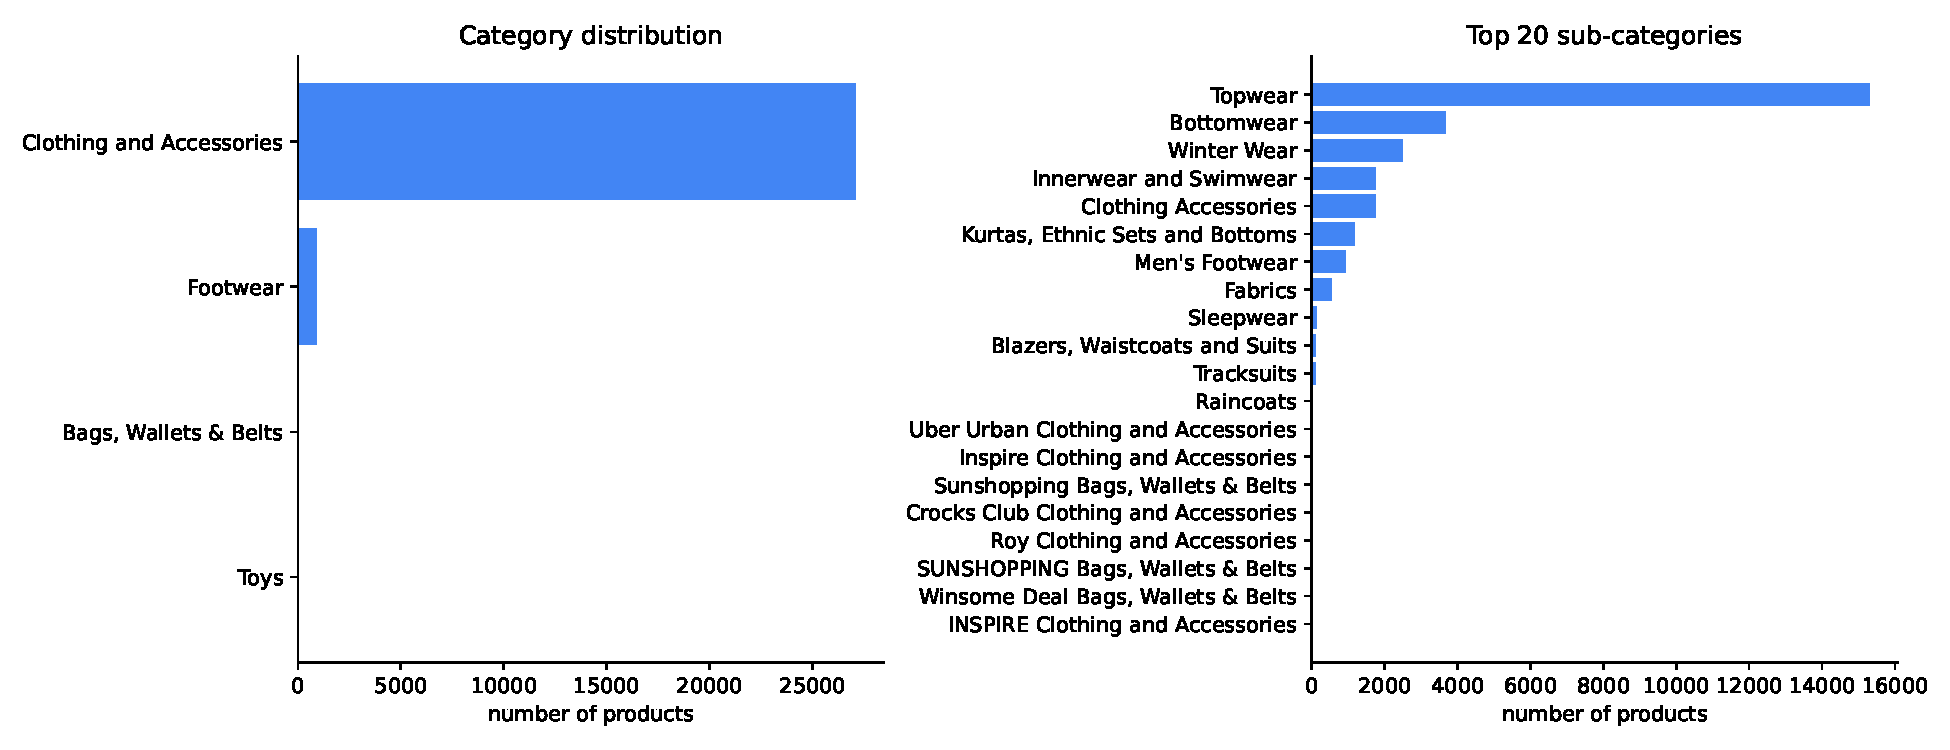
\includegraphics[width=\linewidth]{category_breakdown.pdf}
  \caption{Products per category and per sub-category (top 20).}
  \label{fig:categories}
\end{figure}

\paragraph{Brands and sellers.} Both have a long tail: 324 brands and 534
sellers, and the largest of each (seller \emph{RetailNet}, about 1{,}400
products, 5.3\%; brand \emph{ECKO Unl}, 3.6\%) holds only a small share, and the
top 20 of each cover about 40\% of products (\cref{fig:brands}). Brand names are truncated in the source data (\emph{Pu},
\emph{True Bl}, \emph{V}), while seller names are complete
(\emph{ArvindTrueBlue}). A query for the full brand name will therefore not match
the brand field, so brand matches will be less useful than its distinctiveness
suggests.

\begin{figure}[htbp]
  \centering
  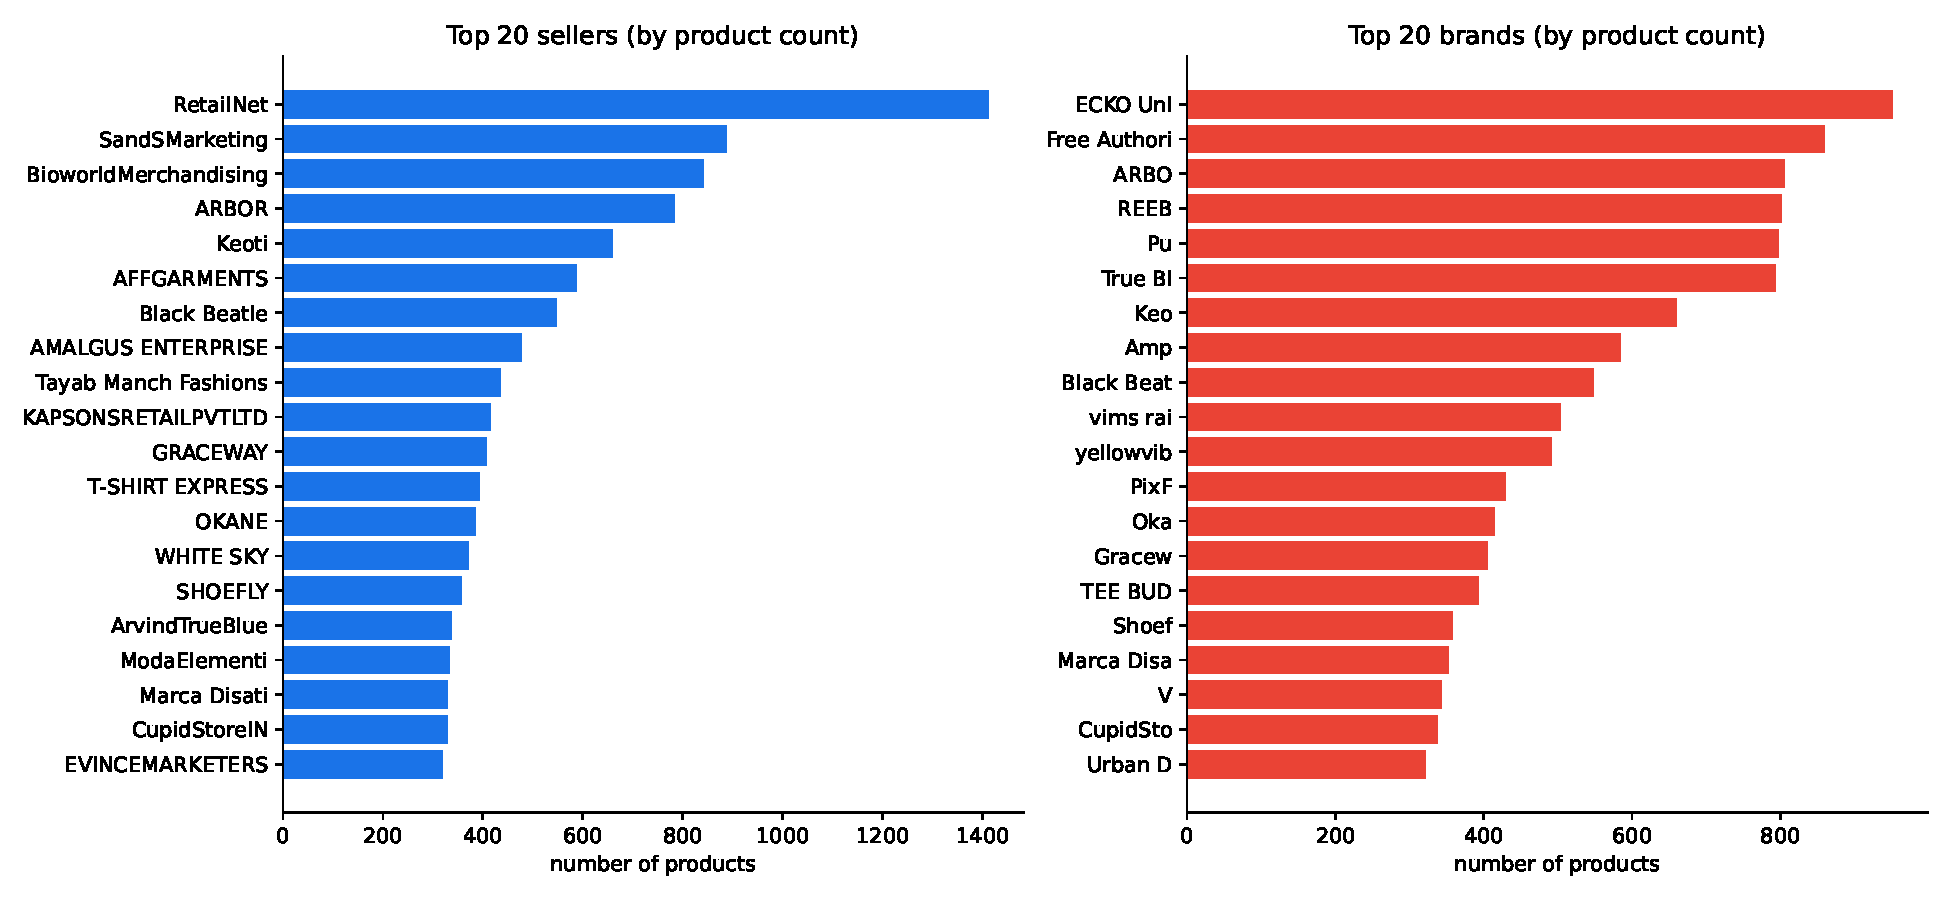
\includegraphics[width=\linewidth]{top_sellers_brands.pdf}
  \caption{The 20 sellers and brands with the most products.}
  \label{fig:brands}
\end{figure}

\paragraph{Prices and discounts.} Prices are right-skewed (\cref{fig:prices}).
The median selling price is INR~545 (half of products between 390 and 820), while
the median actual price is INR~1{,}199. Almost every product is discounted, and
heavily: the median discount is 53\%, half of products are between 40\% and 63\%
off, and the maximum is 87\%. The actual price therefore acts as a reference
price; the selling price is what the user pays and the one to filter on.

\begin{figure}[htbp]
  \centering
  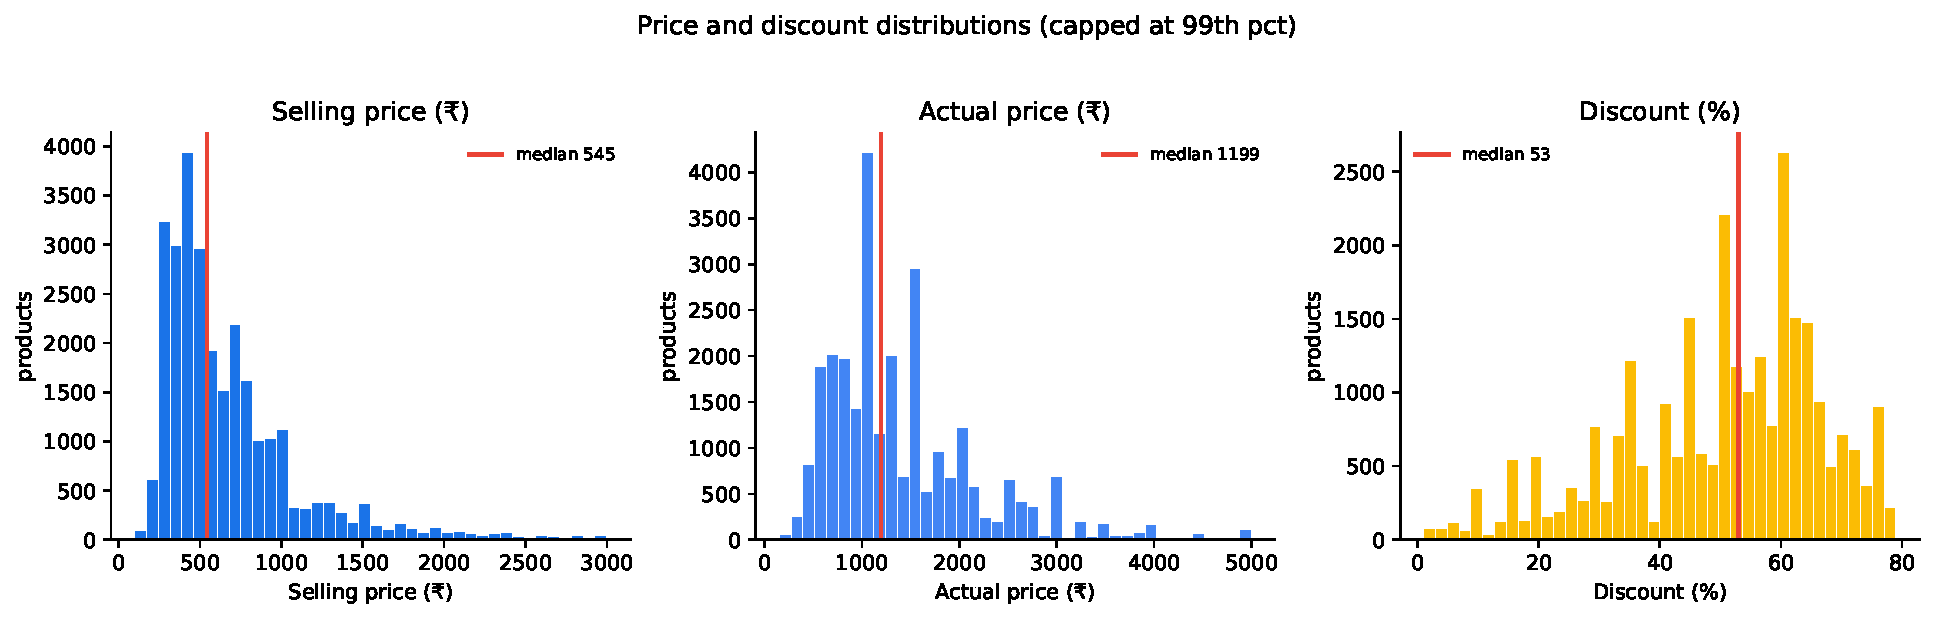
\includegraphics[width=\linewidth]{price_distributions.pdf}
  \caption{Selling price, actual price and discount, capped at the 99th percentile.}
  \label{fig:prices}
\end{figure}

\paragraph{Ratings and stock.} The median rating is 3.8 (mean 3.63, half of
products between 3.2 and 4.1); 16.8\% of rated products are below 3, only 1.3\%
have exactly 5.0, and 8.1\% of products have no rating
(\cref{fig:rating-stock}). Only 5.9\% of products are out of stock, but these
should not be ranked above available ones, so stock will act as a filter or a
penalty.

\begin{figure}[htbp]
  \centering
  \begin{minipage}{0.55\linewidth}
    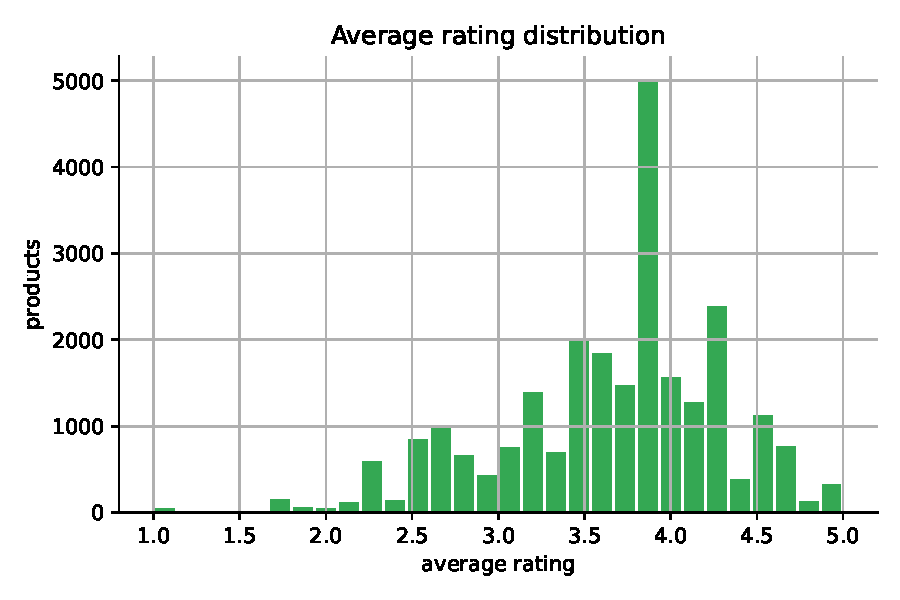
\includegraphics[width=\linewidth]{rating_distribution.pdf}
  \end{minipage}\hfill
  \begin{minipage}{0.42\linewidth}
    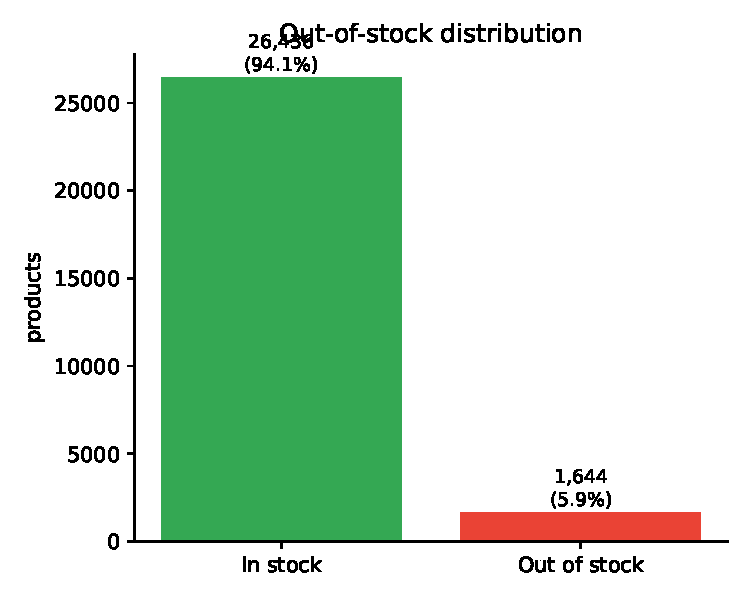
\includegraphics[width=\linewidth]{out_of_stock.pdf}
  \end{minipage}
  \caption{Average rating (left) and stock (right).}
  \label{fig:rating-stock}
\end{figure}

\paragraph{Rankings by a single field.} Sorting by one field shows why none of
them works alone as a ranking. The top products by rating are all ties at 5.0,
and since the dataset has no review counts we cannot tell whether a 5.0 comes
from one review or from thousands. The most discounted products are cheap
t-shirts at 84--87\% off (INR~128 instead of 998), and the most expensive are
suits and jackets at INR~12{,}999. Rating, discount and price are useful signals
on top of text relevance, which is how Part~3 will use them, but not as rankings
by themselves.

\section{Conclusions}

The prepared corpus keeps every field a result must show, with numbers parsed and
missing values kept as missing, plus one list of terms for each of the four
searchable fields. Our main decisions are:

\begin{itemize}
  \item \textbf{One pipeline for documents and queries.} Repairing and normalising
    the text, unifying spelling variants, removing stop words and stemming shrink
    the title vocabulary by 32\% and the description vocabulary by 52\%, and make
    query words such as \emph{women's}, \emph{t-shirt} or \emph{sleeves} match the
    way products write them.
  \item \textbf{Title, description, product details and brand are searched;
    category, sub-category and seller are filters.} Product details are needed:
    without them, 2 of the 13 relevant products of the first validation query miss
    a query word. Category barely varies (96.6\% of products share one value) and
    never contains a query word, so it only works as a filter.
  \item \textbf{Numbers are not terms.} Prices, discount, rating and stock serve as
    filters, as signals for our ranking score in Part~3, and as information on the
    results page.
\end{itemize}

The analysis also shows what to expect when indexing and ranking. Titles are short
and follow a template, and 40\% of products have no description, so many products
have nearly identical text, and document length varies mostly with the
description. The most frequent terms (\emph{tshirt}, \emph{women}, \emph{men},
\emph{cotton}) include most words of the validation queries, so TF-IDF will rank
mainly by the rarer garment words. No numeric field ranks well on its own: the
best-rated products tie at 5.0 with no review counts to separate them, and almost
every product is discounted. Finally, the data has problems that the next parts
must handle: truncated brand names, noisy sub-category values, and validation
labels that do not always contain the literal query words (only 6 of the 10
relevant products for \emph{men slim jeans blue} contain \emph{slim}). An
off-the-shelf entity recogniser mislabels most product titles, so we rely on the
structured fields instead.

\section*{Use of AI tools}

% Check this with the group and add any other AI use before submitting.
We used Claude (Anthropic), through Claude Code, to review the notebook and this
report. It helped write the code production and debugging, and helped draft this report from the
notebook outputs. We checked every number against the notebook outputs and
reviewed and edited the text ourselves.

\bibliographystyle{plain}
\bibliography{refs}

\end{document}
